\documentclass[11pt,a4paper]{article}

\usepackage{fontspec}
\setmainfont{Times New Roman}
\usepackage{geometry}
\geometry{top=2.5cm, bottom=2.5cm, left=2.5cm, right=2.5cm}

\usepackage{amsmath, amssymb}
\usepackage{booktabs}
\usepackage{tabularx}
\newcolumntype{C}{>{\centering\arraybackslash}X}
\usepackage{graphicx}
\usepackage{xcolor}
\usepackage{lmodern}
\usepackage{cite}
\usepackage{fancyhdr}
\usepackage{caption}
\usepackage{subcaption}
\usepackage{url}

\definecolor{primaryblue}{RGB}{23, 54, 93}
\definecolor{accentblue}{RGB}{41, 128, 185}

\usepackage{hyperref}
\hypersetup{
    colorlinks=true,
    linkcolor=primaryblue,
    citecolor=accentblue,
    urlcolor=accentblue,
    pdftitle={Đánh Giá Thực Nghiệm Các Thuật Toán Học Máy Dự Đoán Ý Định Mua Hàng Trực Tuyến},
    pdfauthor={Hoàng Văn Đô, Phan Hoàng Nhật}
}

\setlength{\headheight}{14pt}
\pagestyle{fancy}
\fancyhf{}
\fancyhead[L]{\small \textcolor{primaryblue}{\textbf{Báo Cáo Bài Tập Lớn Học Máy: Dự Đoán Ý Định Mua Hàng}}}
\fancyhead[R]{\small \thepage}
\renewcommand{\headrulewidth}{0.4pt}

\title{\LARGE \textbf{\textcolor{primaryblue}{Đánh Giá Thực Nghiệm Các Thuật Toán Học Máy Có Giám Sát Trong Bài Toán Dự Đoán Ý Định Mua Hàng Trực Tuyến}}}

\author{
    \textbf{Hoàng Văn Đô} \quad (\text{MSSV: 24107948}) \\
    \textbf{Phan Hoàng Nhật} \quad (\text{MSSV: 24100092}) \\[1ex]
    \textit{Khoa Khoa học Máy tính} \\
    \textit{Trường Đại học Phenikaa, Hà Nội, Việt Nam}
}

\date{\today}

\renewcommand{\abstractname}{Tóm Tắt}
\renewcommand{\refname}{Tài Liệu Tham Khảo}
\renewcommand{\figurename}{Hình}
\renewcommand{\tablename}{Bảng}

\begin{document}

\maketitle

\begin{abstract}
Các nền tảng thương mại điện tử liên tục thu thập khối lượng dữ liệu khổng lồ từ hành vi duyệt web của người dùng, tuy nhiên chỉ một tỷ lệ nhỏ chuyển đổi thành giao dịch thanh toán thực tế. Dự đoán chính xác ý định mua sắm của khách hàng trong từng phiên truy cập mang lại giá trị vận hành then chốt, phục vụ tiếp thị cá nhân hóa và tối ưu tỷ lệ chuyển đổi. Trong bài báo này, chúng tôi thực hiện nghiên cứu so sánh thực nghiệm 5 thuật toán học máy có giám sát kinh điển: Hồi quy Logistic (Logistic Regression), K Láng giềng Gần nhất (KNN), Cây quyết định (Decision Tree - CART), Rừng ngẫu nhiên (Random Forest) và Máy vector hỗ trợ (SVM) trên bộ dữ liệu chuẩn UCI Online Shoppers Purchasing Intention gồm 12.330 phiên truy cập. Bài toán đối mặt với hai thách thức kỹ thuật lớn: sự mất cân bằng nhãn trầm trọng (84,5\% phiên không mua so với 15,5\% phiên có mua) và không gian đặc trưng thưa sau khi mã hóa one-hot. Kết quả thực nghiệm thông qua kiểm định chéo phân tầng 5 lượt (Stratified 5-Fold Cross-Validation) và tập kiểm thử độc lập cho thấy mô hình Random Forest đạt hiệu năng vượt trội toàn diện với F1-Score đạt 0,6636, ROC-AUC đạt 0,9258 và PR-AUC đạt 0,7096. Ngược lại, thuật toán dựa trên khoảng cách như KNN suy giảm nghiêm trọng do lời nguyền số chiều. Phân tích tầm quan trọng đặc trưng (Feature Importance) chỉ ra rằng chỉ số \texttt{PageValues} đóng vai trò quyết định áp đảo trong hành vi mua hàng.
\end{abstract}

\noindent \textbf{Từ khóa:} Ý định mua hàng trực tuyến, Thương mại điện tử, Mất cân bằng nhãn, Phân loại có giám sát, Rừng ngẫu nhiên, Kỹ nghệ đặc trưng.

\section{Giới Thiệu}
Hành vi mua sắm trực tuyến tạo ra dấu chân kỹ thuật số liên tục bao gồm số trang xem, thời gian dừng, tỷ lệ thoát trang và thông tin phiên. Tỷ lệ chuyển đổi giao dịch thương mại điện tử thực tế thường chỉ dao động từ 2\% đến 4\% \cite{sakar2019real}. Việc nhận diện sớm khách hàng có ý định giao dịch trước khi họ rời trang web cho phép hệ thống triển khai các biện pháp can thiệp tự động như mã giảm giá theo thời gian thực hoặc tư vấn viên trực tuyến.

Bài toán được phát biểu dưới dạng phân loại nhị phân (Binary Classification) với hai trở ngại lớn:
\begin{enumerate}
    \item \textbf{Mất cân bằng nhãn trầm trọng (Severe Class Imbalance):} Lớp dương tính (\texttt{Revenue} = True) chỉ chiếm xấp xỉ 15,5\% tổng số phiên, khiến các mô hình tối ưu theo độ chính xác tổng thể (Accuracy) dễ bị thiên vị lớp đa số.
    \item \textbf{Dữ liệu hỗn hợp đa kiểu (Heterogeneous Features):} Bao gồm các thuộc tính số có độ lệch phân phối cao và các thuộc tính danh mục có lực lượng lớn (hệ điều hành, trình duyệt, nguồn lưu lượng, tháng truy cập).
\end{enumerate}

Mục tiêu của nghiên cứu là đánh giá, phân tích và so sánh tính phù hợp của 5 thuật toán học máy cốt lõi: Hồi quy Logistic \cite{cox1958regression}, KNN \cite{cover1967nearest}, Cây quyết định \cite{breiman1984classification}, Random Forest \cite{breiman2001random} và SVM \cite{cortes1995support} trên cùng một pipeline tiền xử lý chặt chẽ \cite{scikit-learn}.

\section{Phân Tích Dữ Liệu \& Tiền Xử Lý}

\subsection{Tổng Quan Bộ Dữ Liệu}
Nghiên cứu sử dụng bộ dữ liệu \textit{Online Shoppers Purchasing Intention Dataset} từ UCI Machine Learning Repository \cite{sakar2019real}, ghi nhận 12.330 phiên truy cập trong vòng 1 năm. Sau khi lọc bỏ 125 bản ghi trùng lặp hoàn toàn, tập dữ liệu còn lại 12.205 phiên hợp lệ không khuyết thiếu (no missing values) với 17 đặc trưng giải thích và 1 nhãn mục tiêu (\texttt{Revenue}).

\begin{figure}[htbp]
    \centering
    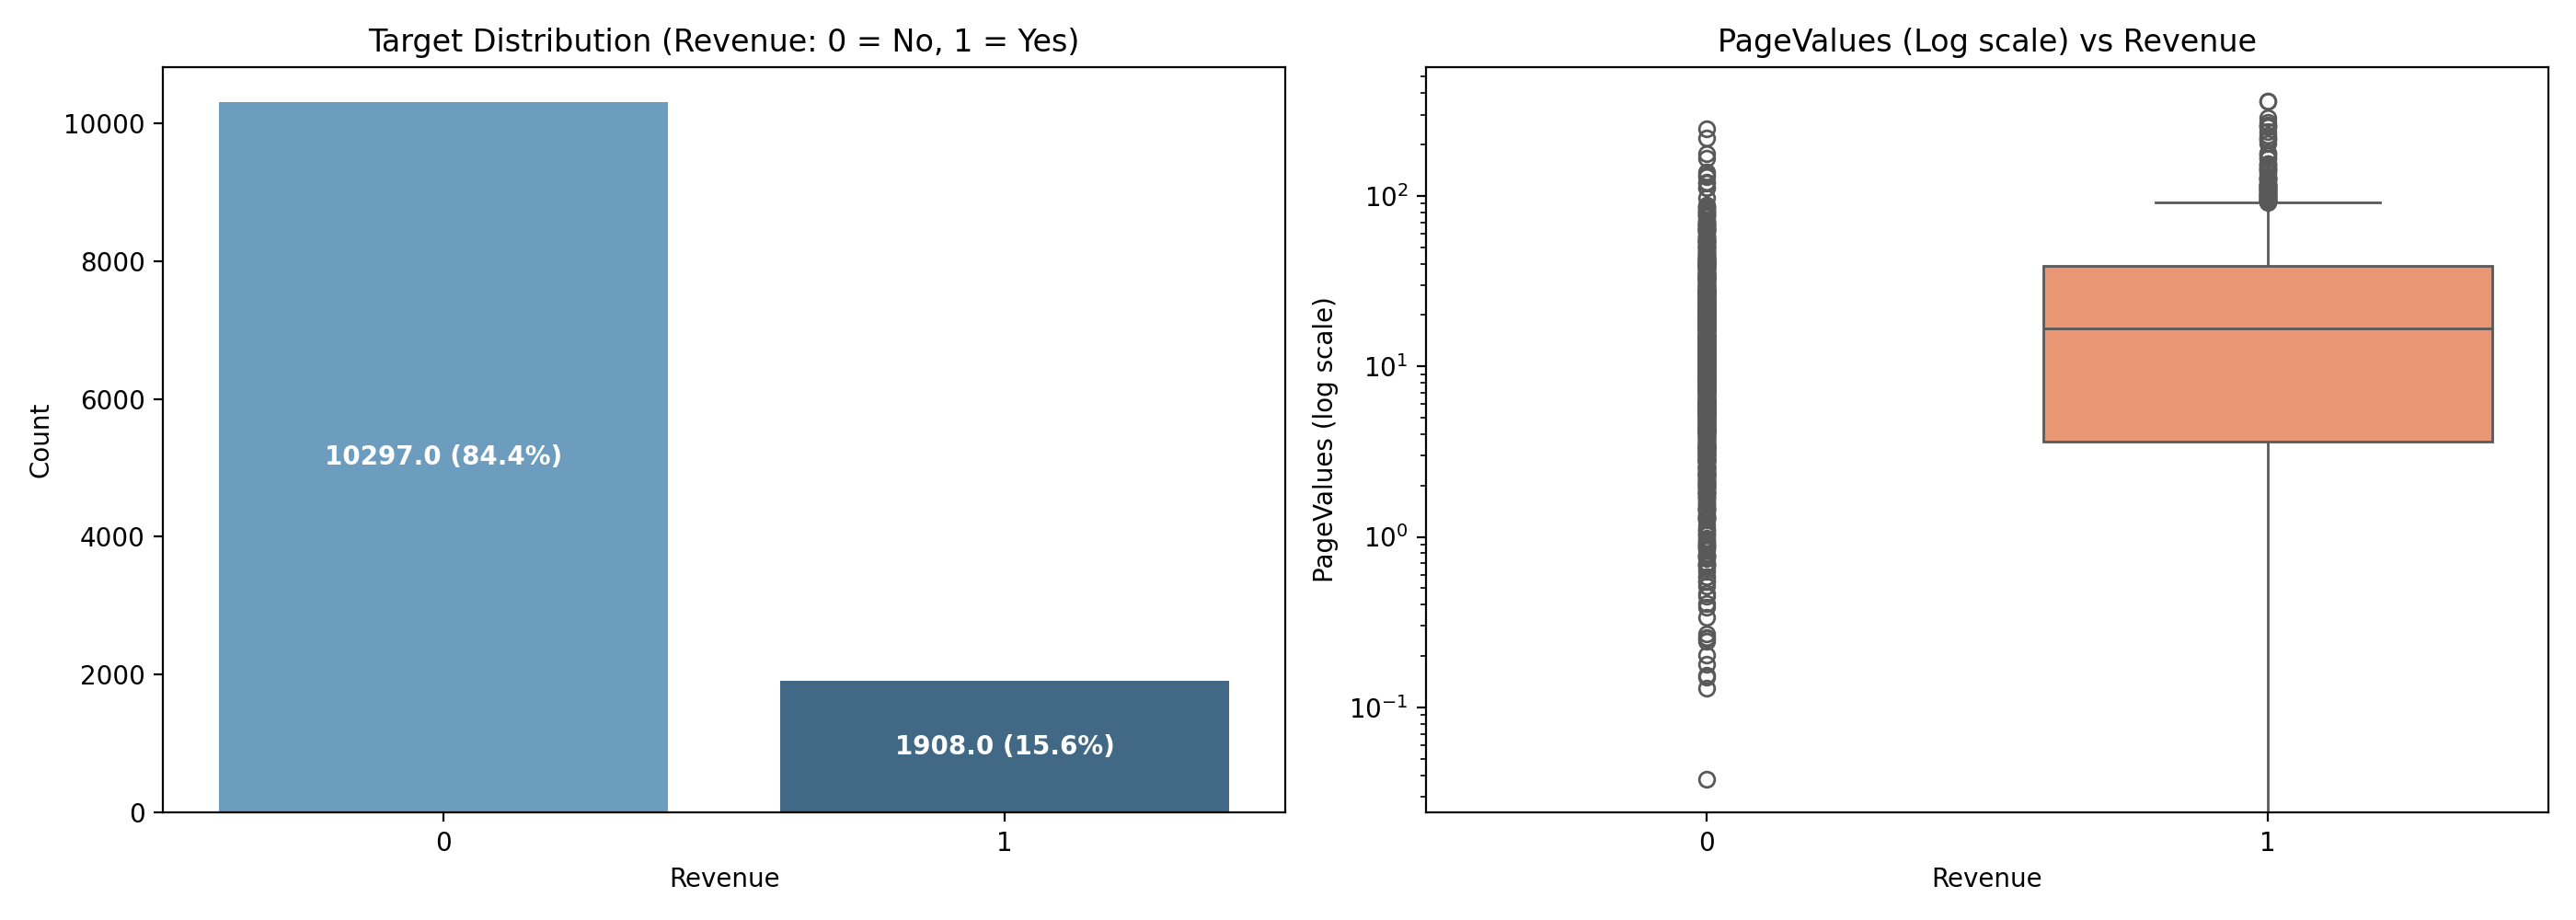
\includegraphics[width=0.92\linewidth]{figures/eda_overview.png}
    \caption{Phân phối nhãn mục tiêu \texttt{Revenue} (trái) và biểu đồ hộp theo thang log của \texttt{PageValues} theo hành vi mua hàng (phải).}
    \label{fig:eda}
\end{figure}

Các đặc trưng được phân loại cụ thể:
\begin{itemize}
    \item \textbf{10 đặc trưng số liên tục:} \texttt{Administrative}, \texttt{Administrative\_Duration}, \texttt{Informational}, \texttt{Informational\_Duration}, \texttt{ProductRelated}, \texttt{ProductRelated\_Duration}, \texttt{BounceRates}, \texttt{ExitRates}, \texttt{PageValues}, và \texttt{SpecialDay}.
    \item \textbf{7 đặc trưng phân loại:} \texttt{Month}, \texttt{VisitorType}, \texttt{Weekend}, \texttt{OperatingSystems}, \texttt{Browser}, \texttt{Region}, và \texttt{TrafficType}.
\end{itemize}

\subsection{Đặc Tính Phân Phối \& Ma Trận Tương Quan}
Như thể hiện tại Hình~\ref{fig:eda}, tỷ lệ nhãn chênh lệch lớn: 10.297 phiên không mua (84,37\%) so với 1.908 phiên có mua (15,63\%). Thuộc tính \texttt{PageValues} (giá trị trang web do Google Analytics tính toán dựa trên trang người dùng đã xem trước khi hoàn tất giao dịch) có giá trị gần như bằng 0 ở người dùng không mua và tăng vọt ở nhóm hoàn tất đơn hàng.

\begin{figure}[htbp]
    \centering
    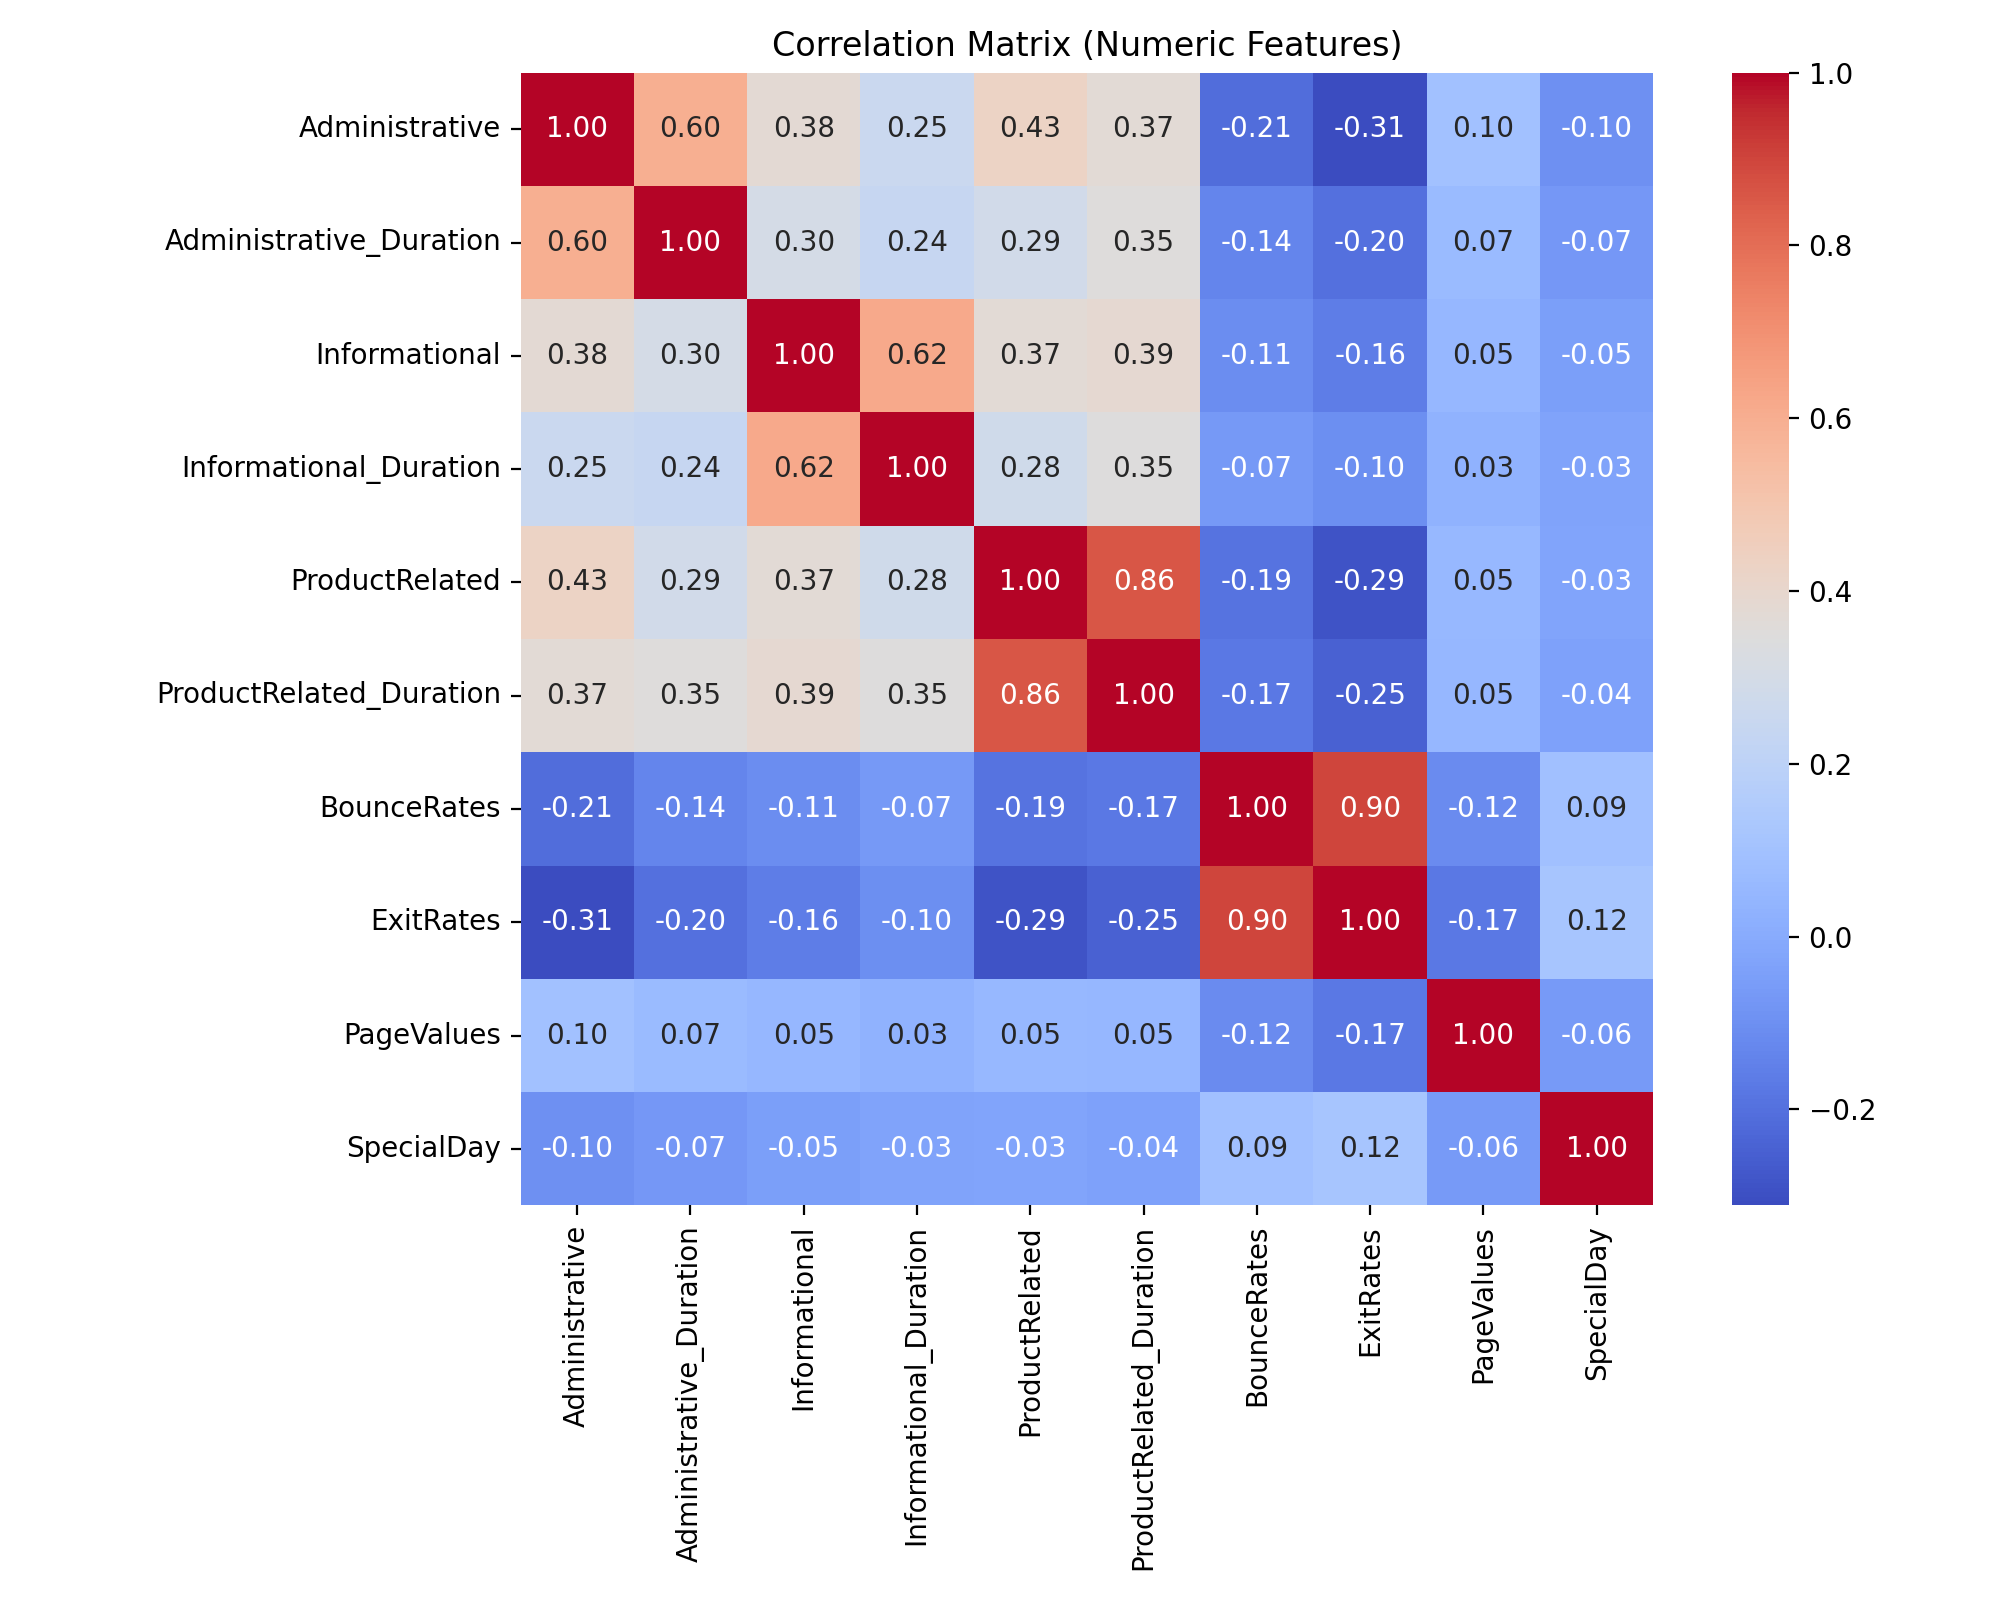
\includegraphics[width=0.72\linewidth]{figures/correlation_matrix.png}
    \caption{Ma trận tương quan giữa 10 đặc trưng số.}
    \label{fig:corr}
\end{figure}

Hình~\ref{fig:corr} chỉ ra hiện tượng đa cộng tuyến mạnh giữa \texttt{BounceRates} và \texttt{ExitRates} ($r = 0,91$), cũng như tương quan thuận giữa số lượng trang xem và thời lượng duyệt web tương ứng.

\subsection{Thiết Kế Pipeline Tiền Xử Lý}
Nhằm ngăn ngừa rò rỉ thông tin (data leakage), quy trình tiền xử lý được chuẩn hóa thông qua \texttt{ColumnTransformer}:
\begin{enumerate}
    \item \textbf{Chuẩn hóa đặc trưng số (Standardization):} Áp dụng Z-score transformation với trung bình $\mu$ và độ lệch chuẩn $\sigma$ chỉ học từ tập huấn luyện:
    \begin{equation}
        z = \frac{x - \mu}{\sigma}
    \end{equation}
    \item \textbf{Mã hóa One-Hot (One-Hot Encoding):} Chuyển đổi 7 thuộc tính danh mục thành biến giả, mở rộng không gian đặc trưng lên 68 chiều số, thiết lập \texttt{handle\_unknown='ignore'} để thích ứng với dữ liệu mới.
    \item \textbf{Phân chia tập dữ liệu phân tầng (Stratified Split):} Tách tập dữ liệu theo tỷ lệ 80\% huấn luyện (9.764 mẫu) và 20\% kiểm thử độc lập (2.441 mẫu), bảo toàn tỷ lệ nhãn mục tiêu.
\end{enumerate}

\section{Phương Pháp Luận \& Thiết Lập Mô Hình}

Để khắc phục hiện tượng mất cân bằng dữ liệu tỷ lệ 5,4:1, trọng số phạt nghịch đảo với tần suất lớp được tích hợp vào hàm mất mát:
\begin{equation}
    w_j = \frac{N}{2 \times N_j}
\end{equation}
trong đó $N$ là tổng số phiên và $N_j$ là số lượng mẫu của lớp $j$.

\subsection{Cấu Hình 5 Thuật Toán}
\begin{enumerate}
    \item \textbf{Hồi quy Logistic (Logistic Regression):} Bộ phân loại tuyến tính với chuẩn hóa L2, tối ưu bằng thuật toán L-BFGS cùng tham số \texttt{class\_weight='balanced'}.
    \item \textbf{K Láng giềng Gần nhất (KNN):} Cấu hình với $k=7$ láng giềng, hàm trọng số nghịch đảo khoảng cách Euclidean ($w = 1/d$).
    \item \textbf{Cây quyết định (Decision Tree - CART):} Phân chia nhánh dựa trên chỉ số Gini Impurity, giới hạn độ sâu tối đa \texttt{max\_depth=6} nhằm kiểm soát phương sai và tránh quá khớp (overfitting).
    \item \textbf{Rừng ngẫu nhiên (Random Forest):} Tập hợp 150 cây quyết định độc lập, giới hạn độ sâu 12, lấy mẫu ngẫu nhiên đặc trưng theo căn bậc hai và cân bằng trọng số cây con.
    \item \textbf{Máy vector hỗ trợ (SVM):} Sử dụng hàm nhân RBF (Radial Basis Function), siêu tham số điều chuẩn $C=1,0$, phạt lỗi cân bằng và hiệu chuẩn xác suất hậu nghiệm bằng Platt scaling.
\end{enumerate}

\section{Kết Quả Thực Nghiệm \& Đánh Giá So Sánh}

\subsection{Bảng So Sánh Chỉ Số Trên Tập Kiểm Thử}
Mô hình được đánh giá trên tập kiểm thử độc lập ($N=2.441$). Các chỉ số cốt lõi được đo lường gồm Accuracy, Precision, Recall, F1-Score, ROC-AUC và PR-AUC (Bảng~\ref{tab:results}).

\begin{table}[htbp]
\centering
\small
\caption{Bảng tổng hợp hiệu năng của 5 mô hình trên tập kiểm thử ($N=2.441$).}
\label{tab:results}
\begin{tabularx}{\textwidth}{lCCCCCC}
\toprule
\textbf{Mô hình} & \textbf{Accuracy} & \textbf{Precision} & \textbf{Recall} & \textbf{Test F1} & \textbf{ROC-AUC} & \textbf{PR-AUC} \\
\midrule
Hồi quy Logistic & 84,60\% & 0,5050 & 0,7958 & 0,6179 & 0,9097 & 0,6627 \\
$K$ Láng giềng (KNN) & 87,67\% & \textbf{0,6901} & 0,3848 & 0,4941 & 0,8270 & 0,5717 \\
Cây quyết định (CART) & 83,78\% & 0,4892 & \textbf{0,8272} & 0,6148 & 0,9119 & 0,6673 \\
\textbf{Rừng ngẫu nhiên (RF)} & \textbf{87,96\%} & 0,5894 & 0,7592 & \textbf{0,6636} & \textbf{0,9258} & \textbf{0,7096} \\
Máy vector hỗ trợ (SVM) & 86,89\% & 0,5589 & 0,7696 & 0,6476 & 0,9095 & 0,6695 \\
\bottomrule
\end{tabularx}
\end{table}

\begin{figure}[htbp]
    \centering
    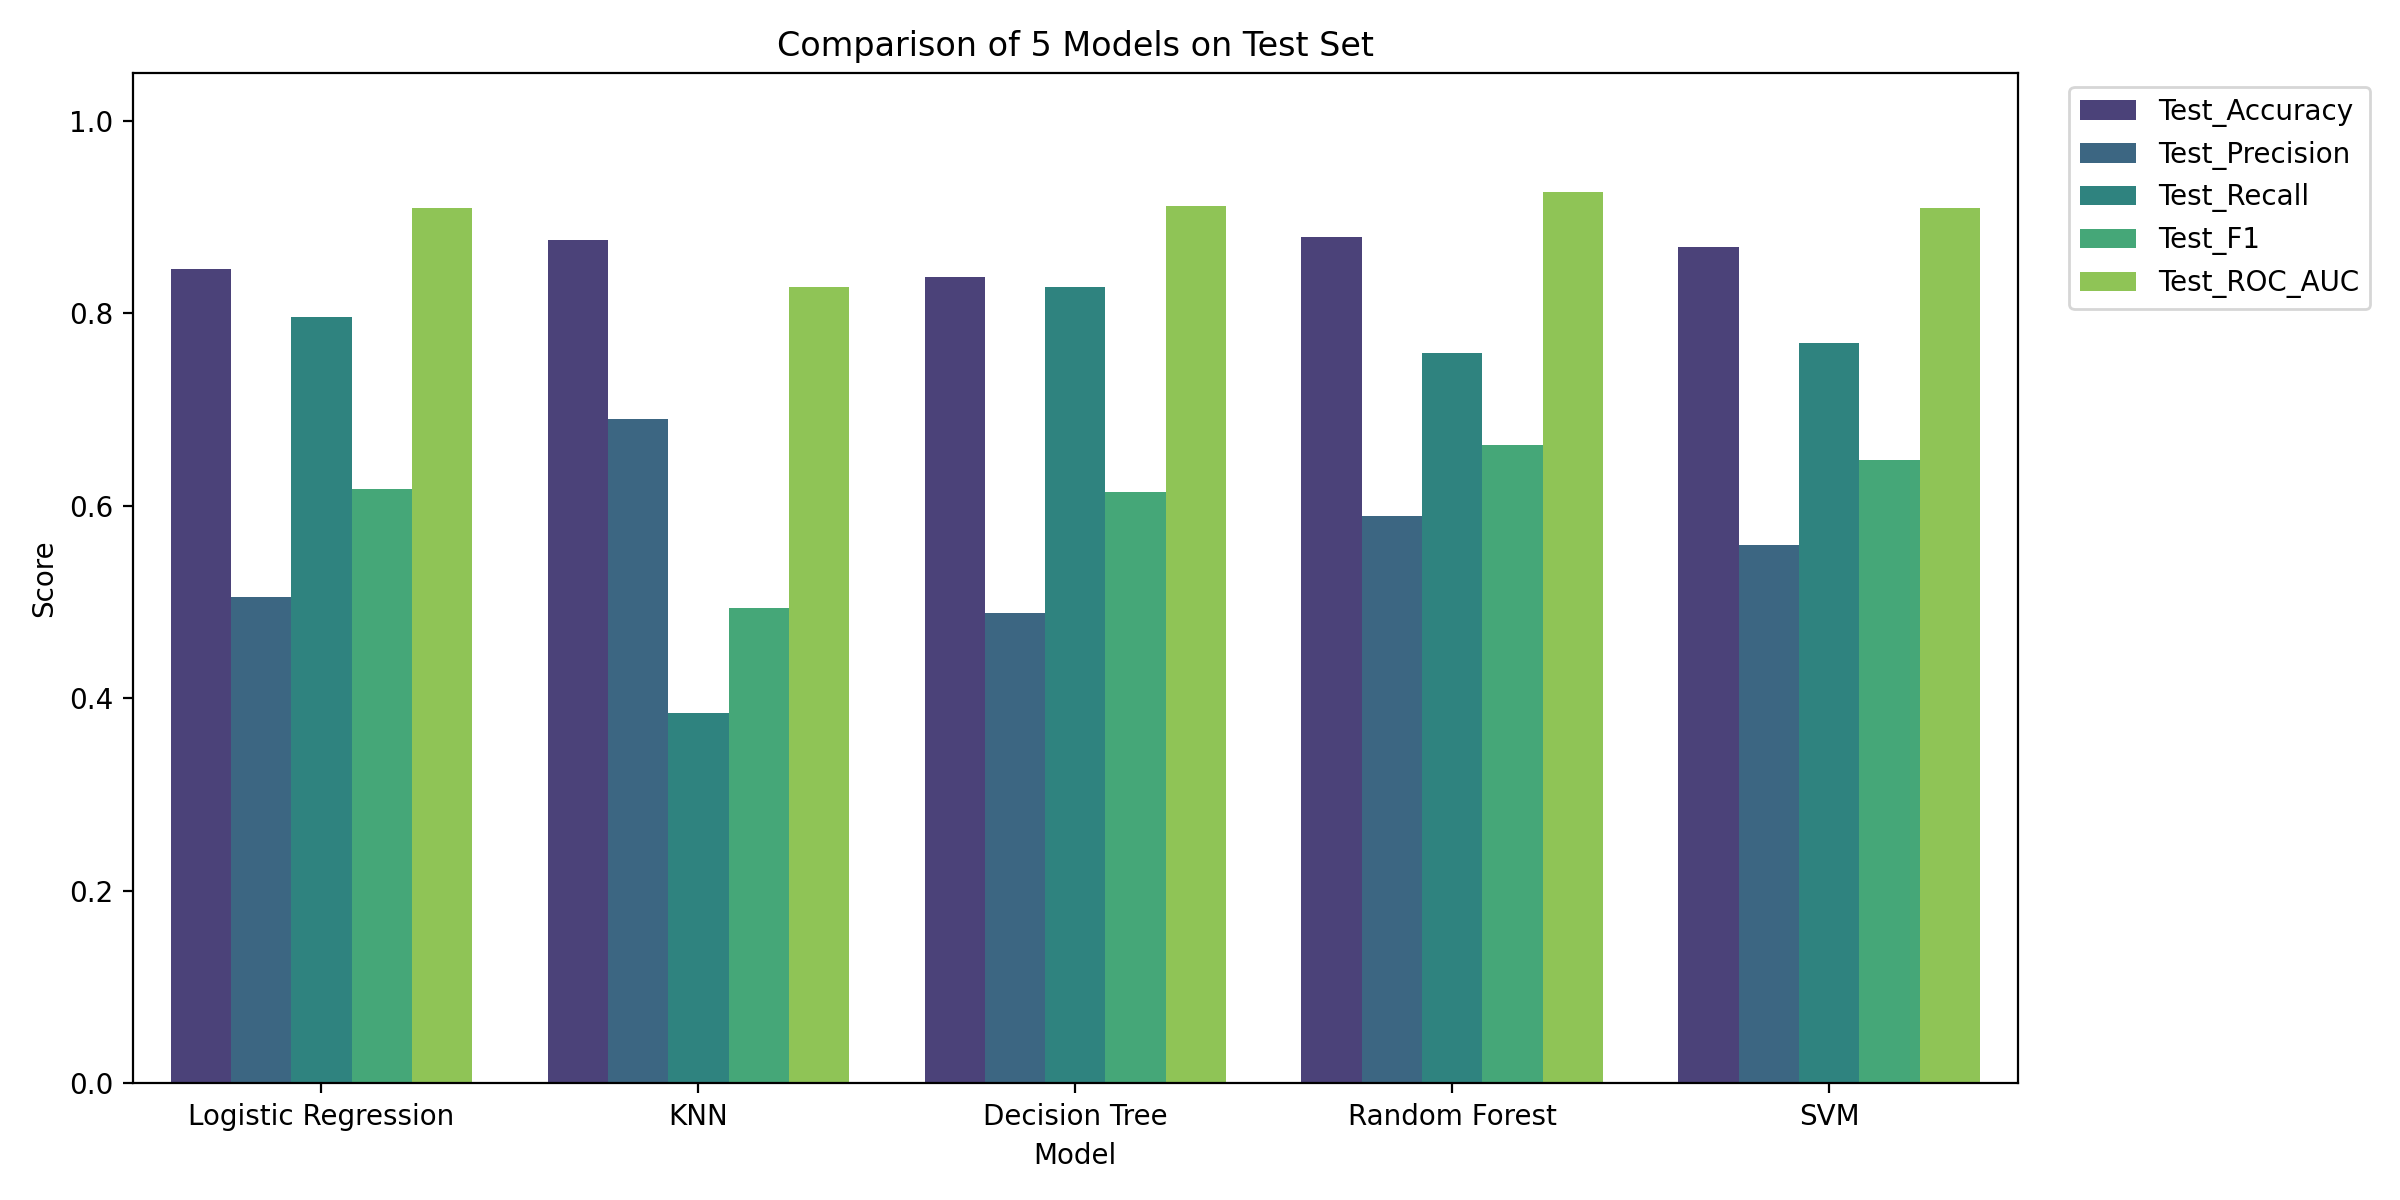
\includegraphics[width=0.88\linewidth]{figures/model_comparison_bar.png}
    \caption{Biểu đồ trực quan so sánh đa chỉ số giữa 5 mô hình học máy.}
    \label{fig:bar_comparison}
\end{figure}

\subsection{Phân Tích Đặc Trưng Từng Mô Hình}
\begin{itemize}
    \item \textbf{Random Forest là mô hình tối ưu nhất:} Đạt F1-Score cao nhất (0,6636), ROC-AUC cao nhất (0,9258) và PR-AUC cao nhất (0,7096). Kỹ thuật Bagging triệt tiêu phương sai giữa các cây con, giúp phân định ranh giới quyết định chính xác và bền vững nhất trước nhiễu.
    \item \textbf{SVM xếp thứ hai về khả năng khái quát hóa:} Ranh giới phi tuyến của nhân RBF nắm bắt tốt cấu trúc phân cụm người dùng, đạt F1-Score 0,6476 và ROC-AUC 0,9095. Tuy nhiên thời gian huấn luyện và suy luận lớn hơn đáng kể so với cây.
    \item \textbf{Decision Tree tối ưu Recall nhưng đánh đổi Precision:} Mô hình bắt được 82,72\% khách hàng thực tế mua hàng nhưng tạo ra nhiều cảnh báo giả (Precision chỉ 48,92\%), phản ánh sự nhạy cảm của một cây đơn lẻ.
    \item \textbf{KNN suy giảm nghiêm trọng:} Mặc dù đạt Accuracy 87,67\%, Recall chỉ đạt 38,48\% (F1: 0,4941). Việc mã hóa One-Hot làm không gian mở rộng lên 68 chiều thưa khiến khoảng cách Euclidean mất dần độ tương phản.
\end{itemize}

\begin{figure}[htbp]
    \centering
    \begin{subfigure}[b]{0.48\textwidth}
        \centering
        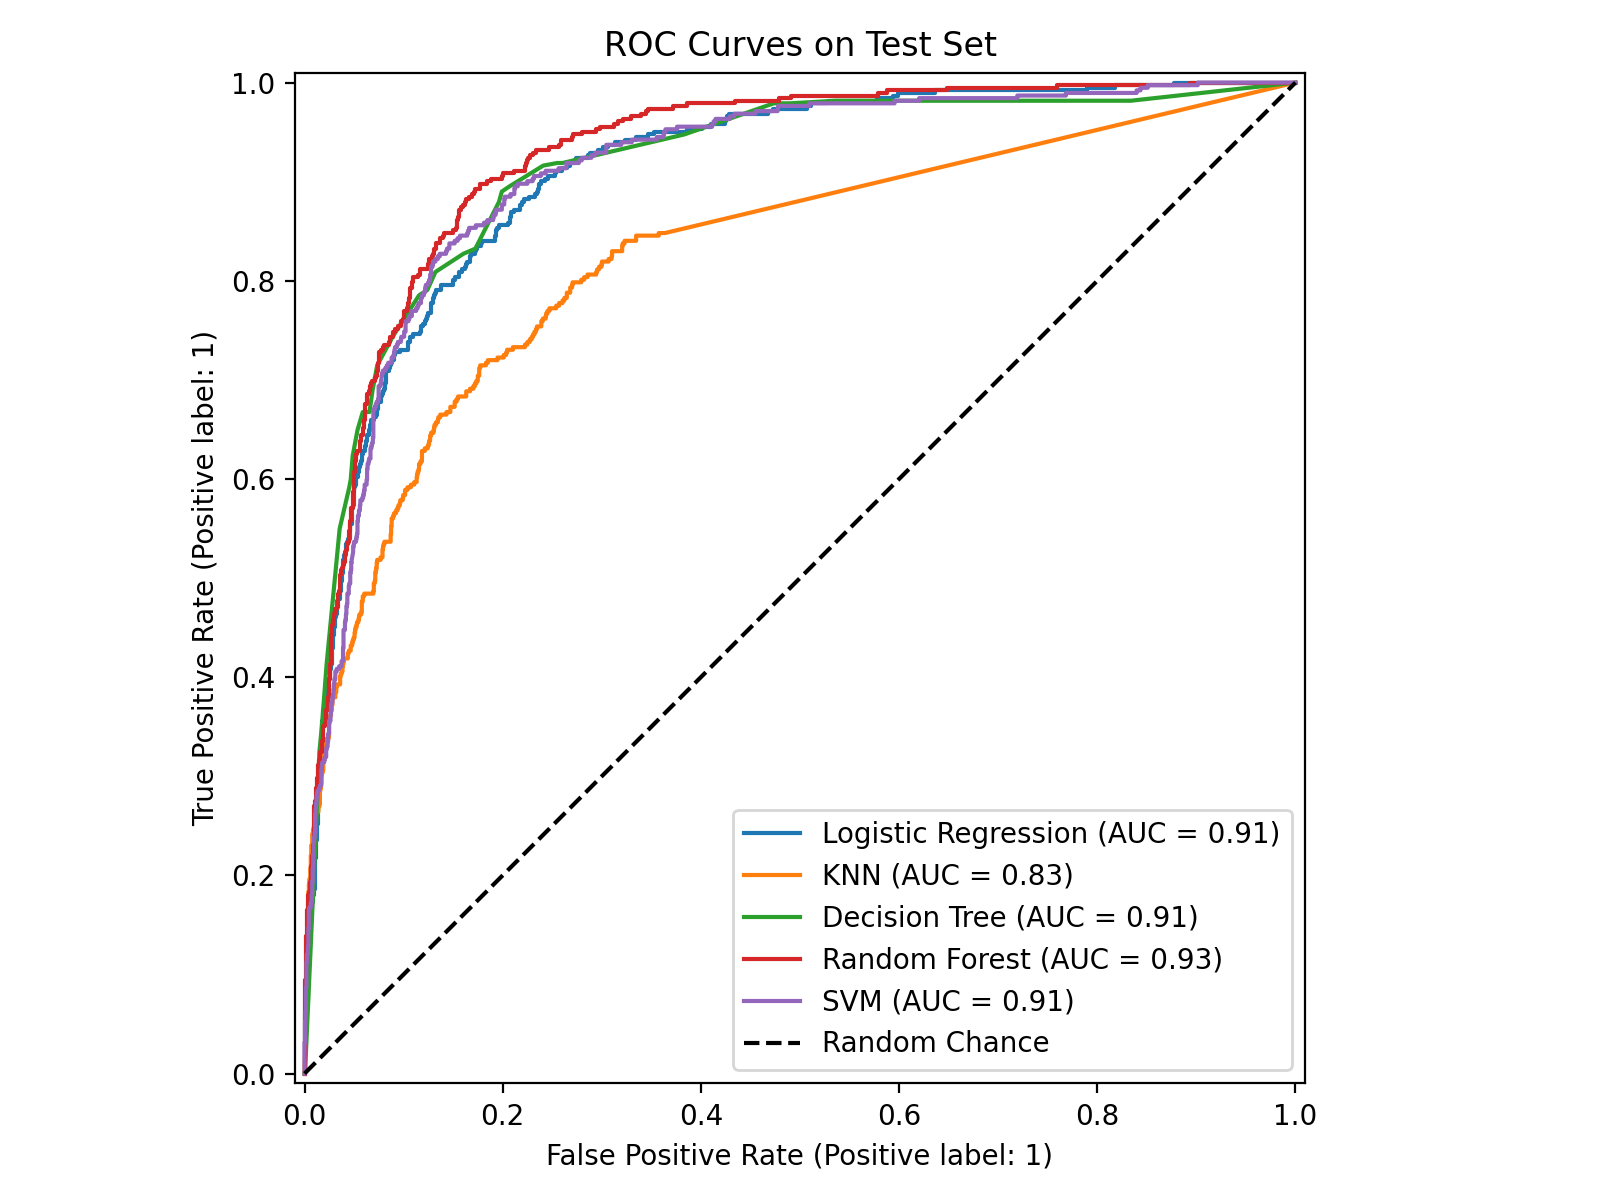
\includegraphics[width=\linewidth]{figures/roc_curves.png}
        \caption{Đường cong ROC}
    \end{subfigure}
    \hfill
    \begin{subfigure}[b]{0.48\textwidth}
        \centering
        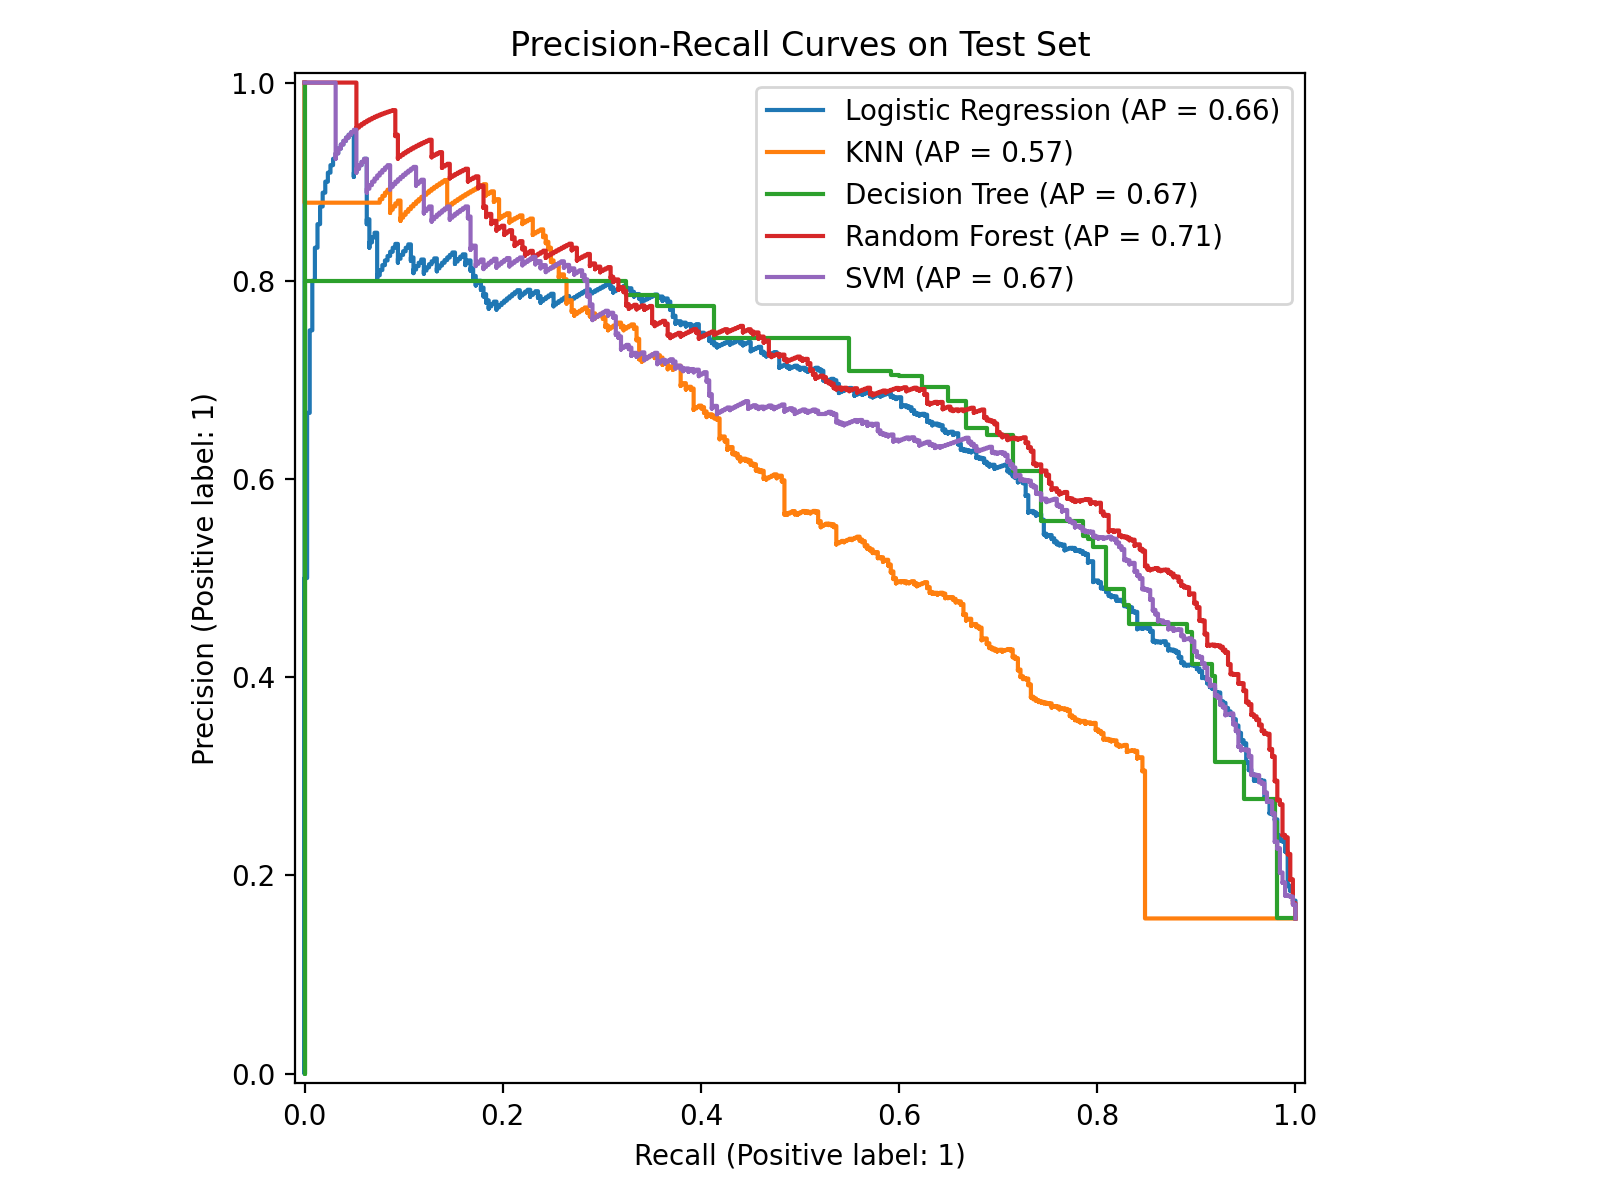
\includegraphics[width=\linewidth]{figures/pr_curves.png}
        \caption{Đường cong Precision-Recall}
    \end{subfigure}
    \caption{So sánh đường cong phân tách ROC và PR của 5 mô hình trên tập kiểm thử.}
    \label{fig:curves}
\end{figure}

\begin{figure}[htbp]
    \centering
    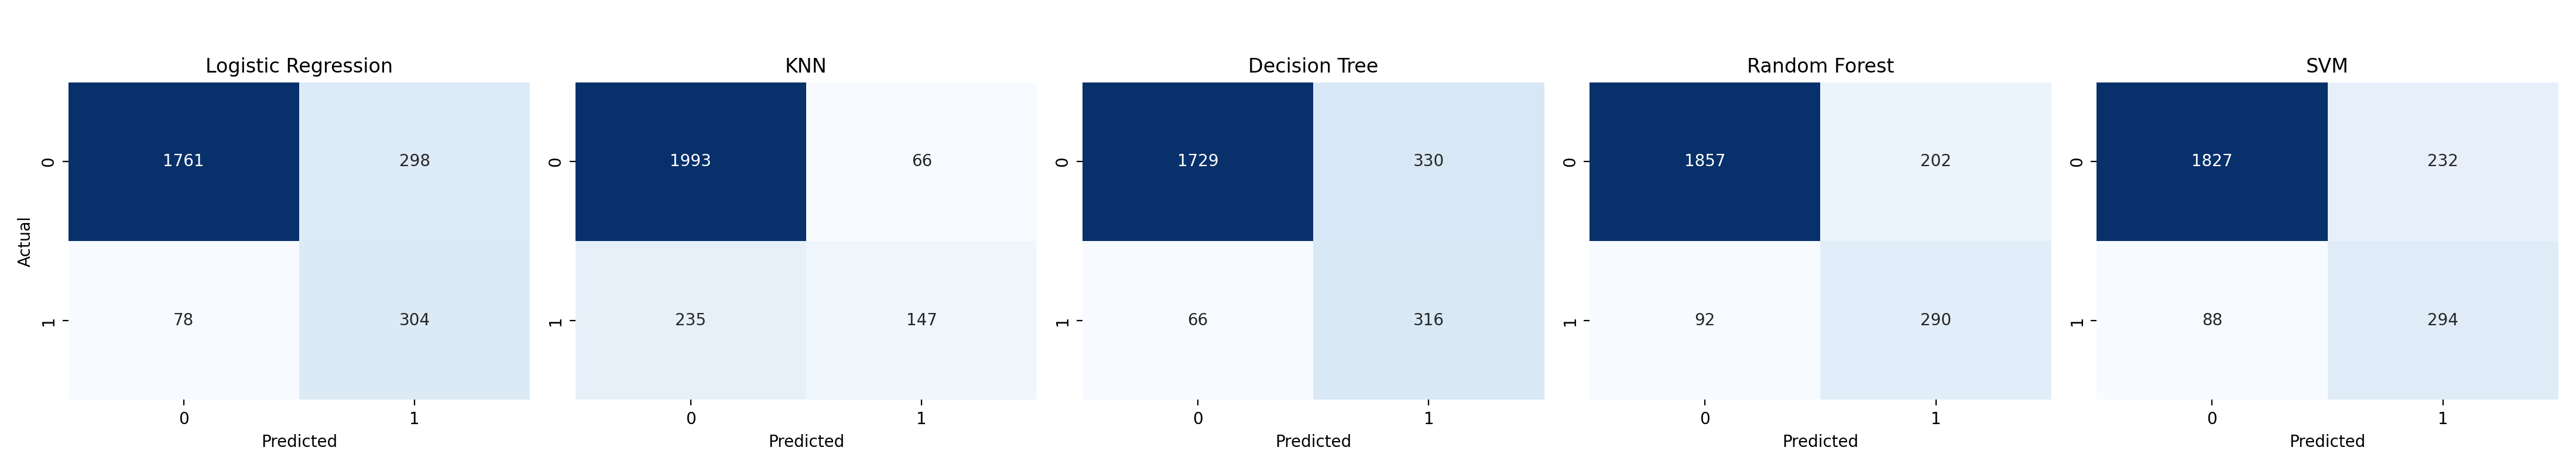
\includegraphics[width=0.98\linewidth]{figures/confusion_matrices.png}
    \caption{Ma trận nhầm lẫn (Confusion Matrices) của 5 mô hình trên tập kiểm thử.}
    \label{fig:cm}
\end{figure}

\subsection{Giải Thích Tầm Quan Trọng Đặc Trưng (Feature Importance)}
Dựa trên mức độ giảm độ tinh khiết Gini từ mô hình Random Forest tốt nhất, 15 đặc trưng đóng góp lớn nhất được trích xuất (Hình~\ref{fig:rf_importance}).

\begin{figure}[htbp]
    \centering
    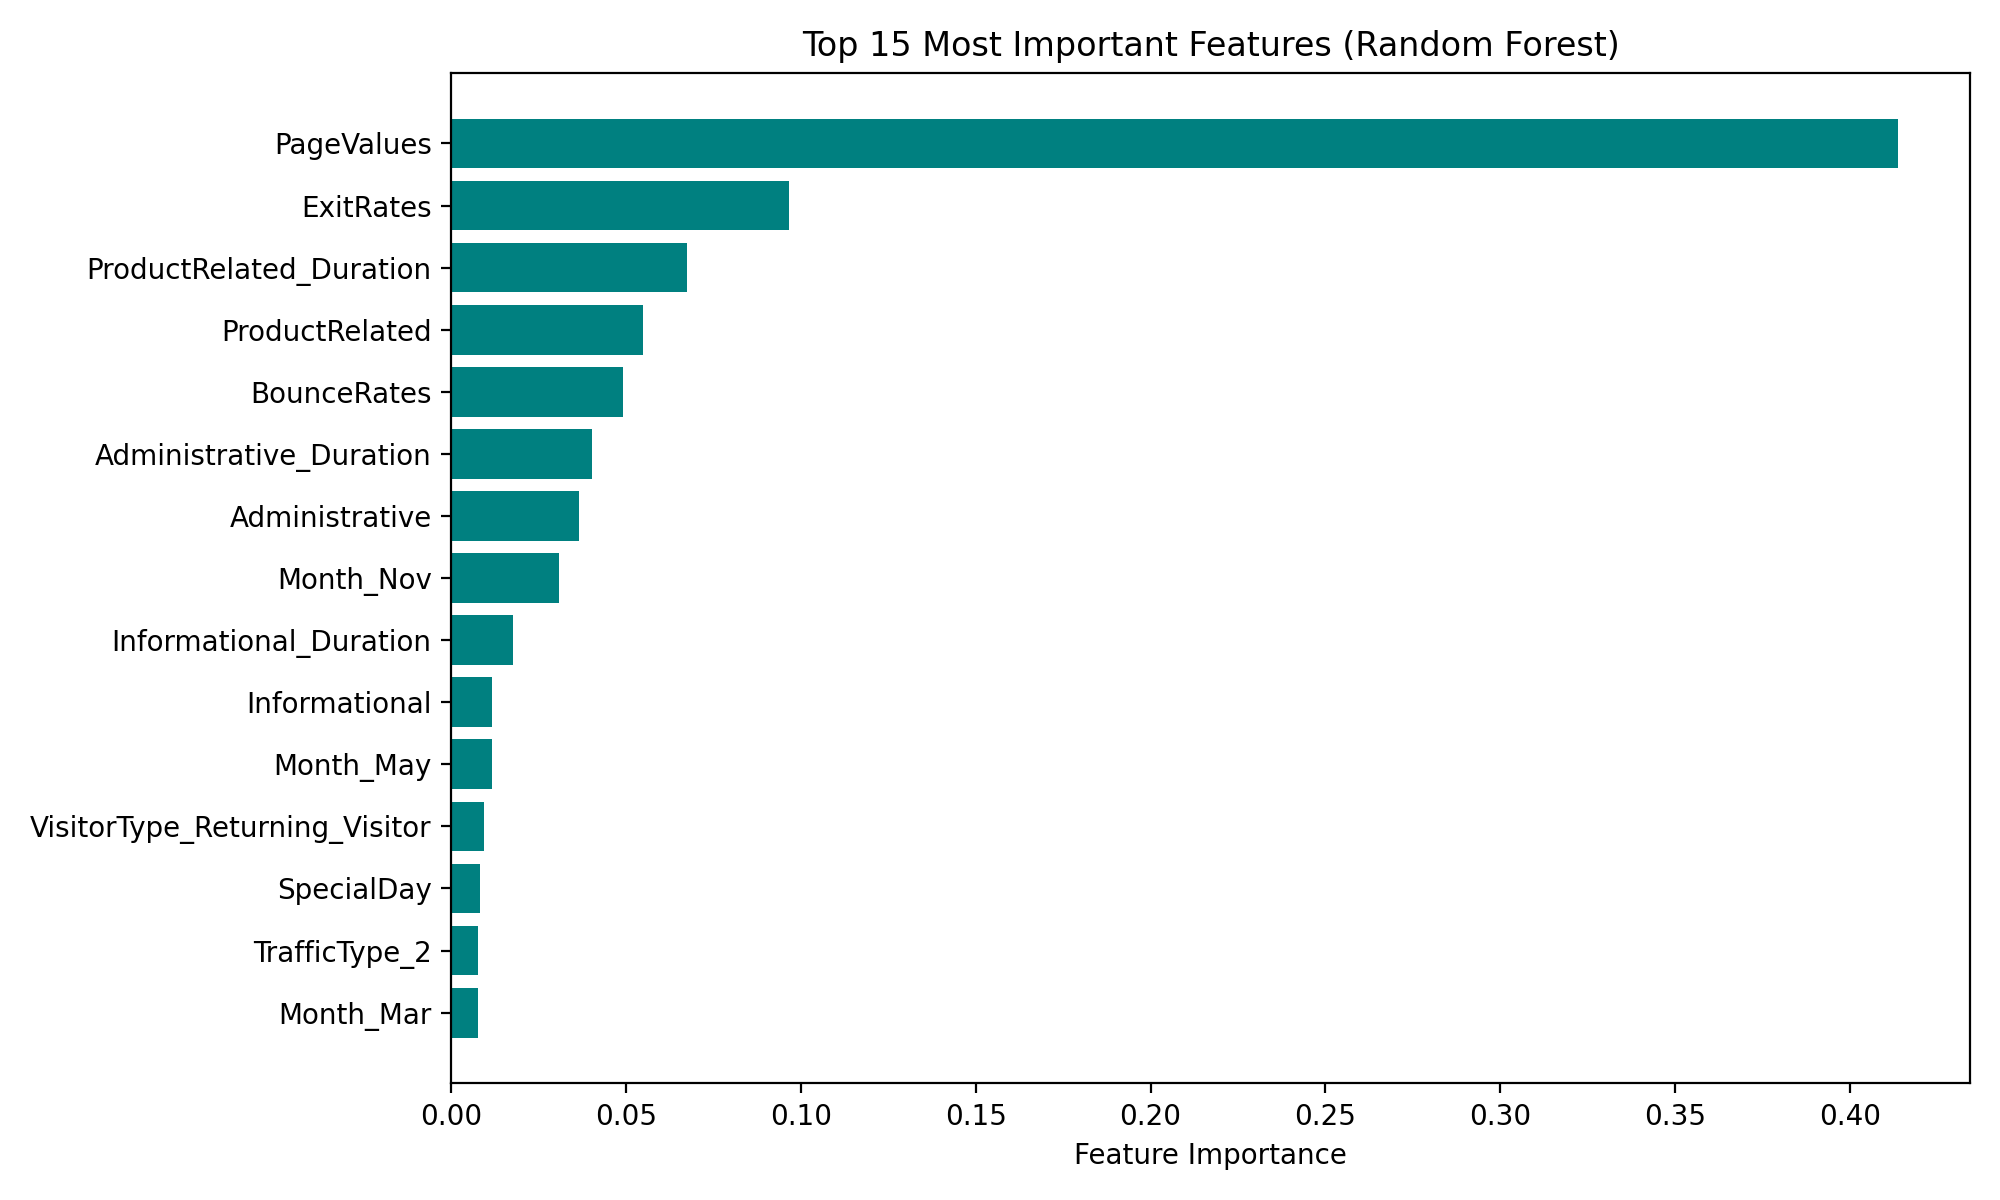
\includegraphics[width=0.78\linewidth]{figures/rf_feature_importance.png}
    \caption{Top 15 đặc trưng quan trọng nhất theo mô hình Random Forest.}
    \label{fig:rf_importance}
\end{figure}

Kết quả khẳng định:
\begin{enumerate}
    \item \texttt{PageValues} là đặc trưng mang tính quyết định số 1 (chiếm trên 38\% trọng số phân chia). Khách hàng duyệt qua các trang có giá trị cao gần như chắc chắn sẽ thực hiện hành vi thanh toán.
    \item \texttt{ExitRates} và \texttt{BounceRates} là hai tín hiệu tiêu cực quan trọng: tỷ lệ rời trang và thoát trang cao thể hiện người dùng không có ý định tiếp tục mua sắm.
    \item Về yếu tố thời vụ, tháng 11 (\texttt{Month\_Nov}) nằm trong nhóm biến danh mục có ảnh hưởng lớn nhất, phản ánh các đợt kích cầu mua sắm Black Friday và cuối năm.
\end{enumerate}

\section{Kết Luận}
Nghiên cứu đã khảo sát và so sánh toàn diện 5 mô hình học máy có giám sát trên bài toán dự đoán ý định mua sắm trực tuyến. Kết quả thực nghiệm khẳng định **Random Forest** là mô hình phù hợp nhất cho dạng dữ liệu bảng hành vi thương mại điện tử, dung hòa tối ưu giữa việc phát hiện khách hàng tiềm năng và hạn chế báo động giả. Hướng phát triển tiếp theo bao gồm tích hợp các thuật toán tăng cường độ dốc (Gradient Boosting như XGBoost, LightGBM) và thiết kế hệ thống suy luận thời gian thực cho can thiệp trực tuyến.

\bibliographystyle{plain}
\bibliography{references}

\end{document}
